\chapter{Calendrier et répartition des tâches}

%============= Calendrier ===================
\section{Calendrier}

	Nous travaillons sur la base d'objectifs d'une durée de 2 semaines maximum. Cela permet de faire un point toutes les 2 semaines avec le responsable du PAO, M. Guerrero, afin d'orienter les objectifs suivants.

% ============= Répartition des tâches ===================
\section{Répartition des tâches}
	Les phases du PAO ont été réalisées en peer-programming, c'est-à-dire en binôme sur une même tache. Cela était indispensable pour la mise en place d'un environnement de développement viable. En effet, il a fallu rechercher et prendre en main les différents outils pour avoir une base stable et commune, puis tester les différentes implémentations en situation réelle avec le drone.

	\begin{figure}
	\hspace{-1cm}
	\begin{tabular}{|@{}l@{}l}
		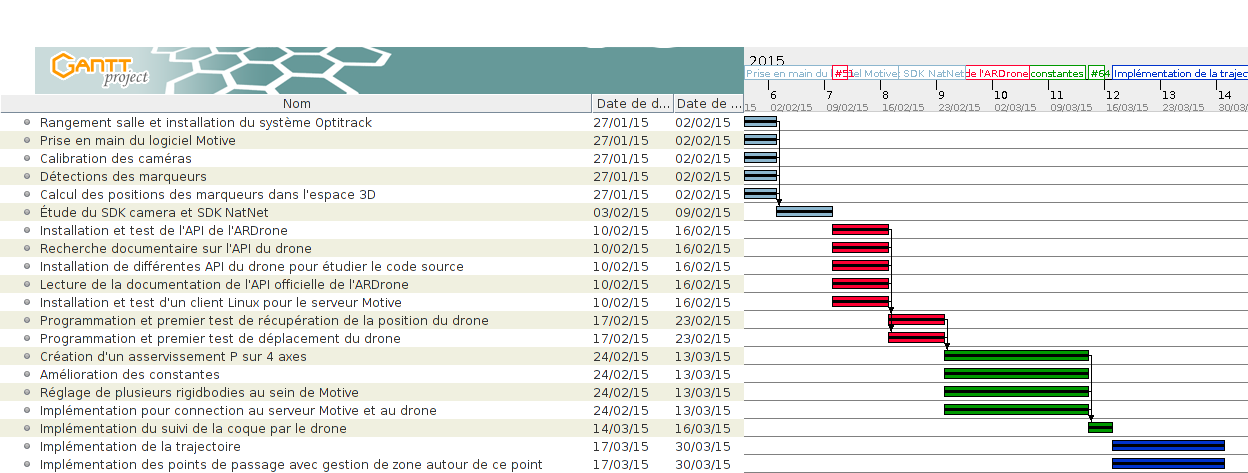
\includegraphics[width=24cm,angle=90]{images/calendrier.png}
	% &
	% 	\includegraphics[width=24cm,angle=90]{images/repartitionCharge.png}
	 \end{tabular}
	 \caption{Planning}
	 \end{figure}
